\documentclass[conference,letterpaper]{IEEEtran}
\IEEEoverridecommandlockouts
\usepackage[T1]{fontenc}
\usepackage{cite}
\usepackage{amsmath,amssymb}
\usepackage{graphicx}
\usepackage{booktabs,tabularx,array,multirow}
\usepackage{xcolor}
\usepackage{tikz}
\usetikzlibrary{arrows.meta,positioning,calc,fit,backgrounds}
\usepackage{pgfplots}
\pgfplotsset{compat=1.18}
\usepackage{listings}
\usepackage{url}
\usepackage[hidelinks]{hyperref}
\hypersetup{pdftitle={GraphRAG over Cyber Threat Reports: Grounding Language-Model Answers in a Neo4j Knowledge Graph of AnnoCTR and MITRE ATT\&CK}, pdfauthor={Shane Waldrop}}

% ---------------------------------------------------------------- colors (diagrams and charts)
\definecolor{ink}{HTML}{1F2A44}
\definecolor{attc}{HTML}{3B5B92}
\definecolor{attf}{HTML}{E8EFF9}
\definecolor{txtc}{HTML}{B5651D}
\definecolor{txtf}{HTML}{FDF0E2}
\definecolor{evalc}{HTML}{3C7A50}
\definecolor{evalf}{HTML}{E6F3EA}
\definecolor{rulec}{HTML}{C9D3E3}
\definecolor{shade}{HTML}{F4F7FB}
\definecolor{sysc}{HTML}{2A78D6}    % chart series 1: GraphRAG / the extraction system
\definecolor{basec}{HTML}{EB6834}   % chart series 2: the baseline
\definecolor{aquac}{HTML}{1BAF7A}
\definecolor{yellowc}{HTML}{EDA100}
\definecolor{magentac}{HTML}{E87BA4}
\definecolor{gridc}{HTML}{E1E0D9}
\definecolor{axisc}{HTML}{C3C2B7}
\definecolor{ink2}{HTML}{52514E}

\newcommand{\code}[1]{\texttt{#1}}
\newcommand{\badge}[1]{\tikz[baseline=(b.base)]\node[circle, fill=ink, text=white, inner sep=0.8pt,
  minimum size=9pt, font=\sffamily\bfseries\tiny](b){#1};}
\tikzset{
  box/.style={draw, rounded corners=2.2pt, align=center, inner sep=2.5pt, font=\sffamily\scriptsize, line width=0.55pt,
    execute at begin node={\hyphenpenalty=10000\exhyphenpenalty=10000\relax}},
  txtbox/.style={box, draw=txtc, fill=txtf},
  attbox/.style={box, draw=attc, fill=attf},
  evalbox/.style={box, draw=evalc, fill=evalf},
  plainbox/.style={box, draw=ink!60, fill=white},
  flow/.style={-{Stealth[length=3.6pt, width=3pt]}, line width=0.55pt, draw=ink!75},
  rel/.style={-{Stealth[length=3.6pt, width=3pt]}, line width=0.55pt},
  elab/.style={font=\sffamily\fontsize{6}{7}\selectfont, fill=white, inner sep=0.8pt},
}
\lstset{basicstyle=\ttfamily\fontsize{7}{8}\selectfont, columns=fullflexible, keepspaces=true, breaklines=true,
  breakatwhitespace=false, frame=single, rulecolor=\color{rulec}, backgroundcolor=\color{shade}, framesep=2pt,
  xleftmargin=2pt, xrightmargin=2pt, aboveskip=4pt, belowskip=2pt, showstringspaces=false, upquote=true,
  postbreak=\mbox{\textcolor{attc}{$\hookrightarrow$}\space}}
\pgfplotsset{
  dotchart/.style={width=\linewidth, axis line style={draw=axisc, line width=0.5pt}, axis x line*=bottom,
    axis y line*=left, y axis line style={draw=none}, major y tick style={draw=none},
    tick style={draw=axisc, line width=0.5pt}, xmajorgrids, grid style={draw=gridc, line width=0.4pt},
    tick label style={font=\sffamily\scriptsize, text=ink2}, label style={font=\sffamily\scriptsize},
    title style={font=\sffamily\scriptsize\bfseries, align=left, anchor=south west, at={(0,1)}, yshift=-1pt},
    yticklabel style={font=\sffamily\scriptsize, text=ink}, clip=false, every axis plot/.append style={line width=0.9pt}},
  sysmark/.style={only marks, mark=*, mark size=1.7pt, color=sysc, error bars/.cd, x dir=both, x explicit,
    error mark=none, error bar style={line width=0.9pt, color=sysc}},
  basemark/.style={only marks, mark=o, mark size=1.7pt, mark options={fill=white, line width=0.9pt}, color=basec,
    error bars/.cd, x dir=both, x explicit, error mark=none, error bar style={line width=0.9pt, color=basec}},
}

\begin{document}

\title{GraphRAG over Cyber Threat Reports: Grounding Language-Model Answers in a Neo4j Knowledge Graph of AnnoCTR and MITRE ATT\&CK}

\author{\IEEEauthorblockN{Shane Waldrop}
\IEEEauthorblockA{\textit{Team CTRL ALT DEFEAT} \textbullet\ CS 6338 Knowledge Engineering\\
Angelo State University, San Angelo, Texas, USA\\
swaldrop2@angelo.edu}}

\maketitle

\begin{abstract}
Cyber threat intelligence (CTI) analysts ask questions joining what a threat report says with what MITRE ATT\&CK (Adversarial Tactics, Techniques, and Common Knowledge) records, such as which mitigations address the most techniques a report describes. Retrieval-augmented generation (RAG) over report text alone cannot answer these multi-hop questions: the connecting facts are not in the text. This paper presents a GraphRAG system that joins ATT\&CK v20.0 (1,785 entries, 20,426 relationships), loaded through a Resource Description Framework (RDF) graph, to 50 expert-annotated AnnoCTR reports in a Neo4j labeled property graph. A large language model (LLM) extracts technique, tactic, group and software mentions under an enforced schema, and a linker resolves them to ATT\&CK by exact name, then by embedding similarity. Mention edges store the evidence sentence, link method, confidence, model and timestamp. Answers draw on report chunks plus graph facts ranked by personalized PageRank; the prompt requires a citation after every statement, and code checks every cited identifier against the context. On 34 held-out test reports, extraction and linking reach a parent-level F1 of 0.709, against 0.442 for exact name matching. On 24 multi-hop questions, GraphRAG names the reference ATT\&CK identifiers with a mean F1 of 0.492, against 0.125 for a text-only baseline, and is rated more complete (3.50 against 1.38 of 5) but less factual (3.17 against 4.63): the baseline mostly declines, while GraphRAG's wrong items follow errors in its own graph (inference). Unsupported statements are rare in both systems (under 2\%), and all 229 GraphRAG citations point into its context.
\end{abstract}

\begin{IEEEkeywords}
GraphRAG, knowledge graphs, cyber threat intelligence, MITRE ATT\&CK, entity linking, Neo4j, personalized PageRank
\end{IEEEkeywords}

% =====================================================================================================================
\section{Introduction}
\textbf{Problem.} A security operations analyst who reads a vendor threat report has to turn its narrative into decisions: which adversary techniques it describes, which threat groups are known to use them, and which mitigations would block the most of them. The report supplies one half of each answer; MITRE ATT\&CK (Adversarial Tactics, Techniques, and Common Knowledge) \cite{strom2020}, a curated public knowledge base of tactics, techniques, groups, software and mitigations, supplies the other. The question ``Which ATT\&CK mitigations address the largest number of the techniques described in report~$X$?'' takes four steps: from the report to the techniques it describes, from each sub-technique to its parent, from each technique to its mitigations, and a count. Retrieval-augmented generation (RAG) \cite{lewis2020}, which retrieves report passages and hands them to a large language model (LLM), finds the right report but not the ATT\&CK relationships. In the evaluation below, a text-only RAG baseline declined 21 of 24 such questions, stating that its context lacked the ATT\&CK information.

\textbf{Domain.} Cyber threat intelligence (CTI) suits a knowledge-graph approach for three reasons. Claims must be verifiable, because analysts act on them, so every answer needs provenance. Both kinds of source exist in public: AnnoCTR \cite{lange2024} annotates 400 threat reports donated by five vendors (Intel 471, Lab52 of S2 Grupo, Proofpoint, QuoIntelligence and Zscaler) and, in 120 of them, links mentions to ATT\&CK; these expert links serve as gold labels (license: Creative Commons Attribution-ShareAlike, CC BY-SA 4.0); ATT\&CK provides the structured side as a versioned STIX (Structured Threat Information Expression) file. And the questions are multi-hop by nature, which is where graph retrieval is expected to help \cite{gutierrez2024,peng2024}.

\textbf{Contributions.} The system, built and evaluated for this project, makes five design choices:
\begin{itemize}
\item A two-source knowledge graph: ATT\&CK v20.0 enters through an RDF/OWL (Resource Description Framework / Web Ontology Language) graph built with rdflib and checked by a SPARQL (SPARQL Protocol and RDF Query Language) count of its classes, then becomes a Neo4j labeled property graph (LPG), joined to report text by extracted and linked mentions whose edges carry full provenance.
\item Schema-enforced LLM extraction and named entity disambiguation (NED) whose threshold was calibrated on a development split before a single run on the test split.
\item Report-anchored GraphRAG, that is, retrieval-augmented generation from a graph \cite{edge2024,peng2024}: personalized PageRank \cite{haveliwala2002} seeded on the nodes a report mentions, summary counts computed in Cypher, and an automatic check that every cited identifier was in the model's context.
\item Graph analytics with Neo4j Graph Data Science (GDS): PageRank \cite{brin1998}, Louvain communities \cite{blondel2008} and FastRP (Fast Random Projection) embeddings \cite{chen2019}, with a topological analysis of the ATT\&CK graph.
\item A reproducible evaluation: every model reply is saved under the \mbox{SHA-256} (Secure Hash Algorithm, 256-bit) hash of its request, so the results can be recomputed from the repository without a new model call, and the scripts behind this paper's tables and figures are in its \code{docs/final} folder; the comparison uses a text-only baseline, blind human ratings, RAGAS (Retrieval Augmented Generation Assessment) \cite{es2024} and 95\% bootstrap intervals \cite{efron1993}.
\end{itemize}
This introduction and Sections~\ref{sec:schema}--\ref{sec:eval} follow the six parts the assignment names: schema and ontology, extraction and ingestion, graph analytics and reasoning, LLM integration, and evaluation. All results are \emph{measured} on the committed data unless marked otherwise; code, data, saved replies and results are in the public repository \url{https://github.com/Wittyusername12/ctrl-alt-defeat-graphrag} (branch \code{build}).

% =====================================================================================================================
\section{Knowledge Graph Schema and Ontology Design}\label{sec:schema}
\subsection{Node labels, relationship types and edge properties}
The graph has eight node labels (Fig.~\ref{fig:schema}). Report and Chunk hold the text. Technique (sub-techniques included), Tactic, Group, Software and Mitigation hold ATT\&CK entries, keyed by their ATT\&CK identifier (ID) in \code{attack\_id}, with the properties \code{name}, \code{aliases}, \code{description}, \code{url} and \code{stix\_id}, plus \code{is\_subtechnique} on Technique, \code{software\_type} (malware or tool) on Software and \code{shortname} on Tactic; the analytics of Section~\ref{sec:gds} add \code{pagerank}, \code{community} and \code{fastrp}. Entity holds the name from a mention the linker left unlinked, either because no ATT\&CK entry matched closely enough or because the model's own confidence fell below the cut-off $c$ (Section~\ref{sec:ned}); it is keyed by category and normalized name, so repeated names merge into one node. Six relationship types connect them (Table~\ref{tab:rels}). Every relationship carries \code{edge\_id}, the identifier an answer cites, and \code{source}, either \code{attack} (recorded by MITRE) or \code{text} (extracted from a report). The loaded graph holds 2,258 nodes: 1,785 ATT\&CK entries, 50 reports (16 dev, 34 test), 149 chunks and 274 Entity nodes.

\begin{figure}[t]\centering
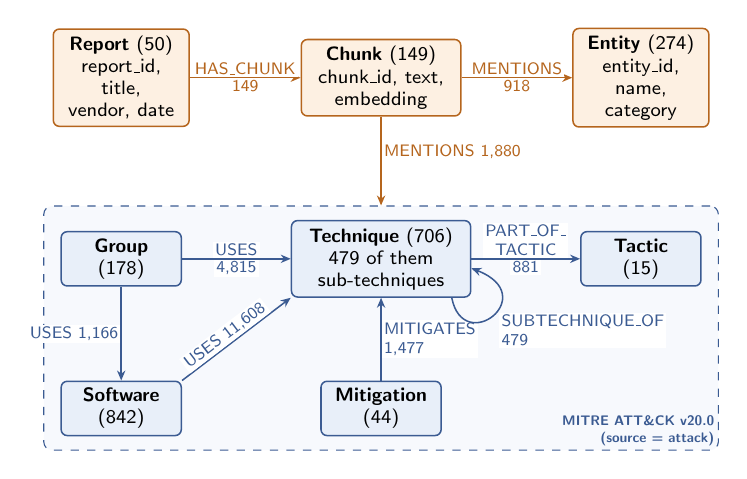
\begin{tikzpicture}[x=1cm, y=1cm]
\node[txtbox, text width=1.55cm] (report) at (0,0) {\textbf{Report} (50)\\report\_id, title,\\vendor, date};
\node[txtbox, text width=1.85cm] (chunk) at (3.3,0) {\textbf{Chunk} (149)\\chunk\_id, text,\\embedding};
\node[txtbox, text width=1.55cm] (entity) at (6.6,0) {\textbf{Entity} (274)\\entity\_id, name,\\category};
\node[attbox, text width=1.35cm] (group) at (0,-2.3) {\textbf{Group}\\(178)};
\node[attbox, text width=2.1cm] (technique) at (3.3,-2.3) {\textbf{Technique} (706)\\479 of them\\sub-techniques};
\node[attbox, text width=1.35cm] (tactic) at (6.6,-2.3) {\textbf{Tactic}\\(15)};
\node[attbox, text width=1.35cm] (software) at (0,-4.2) {\textbf{Software}\\(842)};
\node[attbox, text width=1.35cm] (mitigation) at (3.3,-4.2) {\textbf{Mitigation}\\(44)};
\begin{scope}[on background layer]
\node[draw=attc, dashed, rounded corners=3pt, fill=attf!35, inner xsep=6pt, inner ysep=5pt,
      fit=(group)(technique)(tactic)(software)(mitigation)] (att) {};
\end{scope}
\node[font=\sffamily\tiny\bfseries, text=attc, anchor=south east, inner sep=1.5pt, align=right] at (att.south east)
  {MITRE ATT\&CK v20.0\\(source = attack)};
\draw[rel, txtc] (report) -- node[elab, above, text=txtc]{HAS\_CHUNK} node[elab, below, text=txtc]{149} (chunk);
\draw[rel, txtc] (chunk) -- node[elab, above, text=txtc]{MENTIONS} node[elab, below, text=txtc]{918} (entity);
\draw[rel, txtc] (chunk.south) -- node[elab, right, text=txtc, pos=0.4]{MENTIONS 1,880} (chunk.south |- att.north);
\draw[rel, attc] (group) -- node[elab, above, text=attc]{USES} node[elab, below, text=attc]{4,815} (technique);
\draw[rel, attc] (group) -- node[elab, left, text=attc]{USES 1,166} (software);
\draw[rel, attc] (software.north east) -- node[elab, sloped, above, text=attc, pos=0.45]{USES 11,608} (technique.south west);
\draw[rel, attc] (technique) -- node[elab, above, text=attc, align=center]{PART\_OF\_\\TACTIC} node[elab, below, text=attc]{881} (tactic);
\draw[rel, attc] (mitigation) -- node[elab, right, text=attc, align=left]{MITIGATES\\1,477} (technique);
\draw[rel, attc] ([xshift=-2.5mm]technique.south east) .. controls +(0.15,-0.75) and +(0.9,-0.35) .. ([yshift=-1.2mm]technique.east)
  node[elab, text=attc, anchor=north west, pos=0.55, xshift=1pt, align=left] {SUBTECHNIQUE\_OF\\479};
\end{tikzpicture}
\caption{Knowledge-graph schema with node and relationship counts. Orange: report text and its derived edges (\code{source = text}); blue: ATT\&CK (\code{source = attack}). MENTIONS reaches any ATT\&CK node or an Entity. Besides the 17,589 ATT\&CK USES relationships, 299 USES edges extracted from text join the nodes that a report's group, software and technique mentions link to.}\label{fig:schema}
\end{figure}

\begin{table}[t]\centering\footnotesize
\caption{Relationship types, counts and properties}\label{tab:rels}
\setlength{\tabcolsep}{3pt}
\begin{tabularx}{\linewidth}{@{}>{\raggedright\arraybackslash}p{3.55cm}>{\raggedright\arraybackslash}X@{}}
\toprule
Type: from $\rightarrow$ to (count) & Properties besides \code{edge\_id}, \code{source}\\
\midrule
HAS\_CHUNK: Report $\rightarrow$ Chunk (149) & none\\
MENTIONS: Chunk $\rightarrow$ ATT\&CK node (1,880) or Entity (918) & report\_id, chunk\_id, mention\_text, evidence, category, attack\_name, link\_method, confidence, model\_confidence, model, reply\_key, extracted\\
USES: Software $\rightarrow$ Technique (11,608), Group $\rightarrow$ Technique (4,815), Group $\rightarrow$ Software (1,166); from text (299) & ATT\&CK: stix\_id, description; text: report\_id, chunk\_id, evidence, reply\_key\\
SUBTECHNIQUE\_OF: Technique $\rightarrow$ Technique (479) & stix\_id\\
PART\_OF\_TACTIC: Technique $\rightarrow$ Tactic (881) & none (from kill-chain phases)\\
MITIGATES: Mitigation $\rightarrow$ Technique (1,477) & stix\_id, description\\
\bottomrule
\end{tabularx}
\end{table}

\subsection{Provenance, timestamps and confidence}
Each text-derived MENTIONS edge records where the fact came from and how it was resolved: the report and chunk; the mention text and the whole evidence sentence, both copied by the model and checked by code to occur in the chunk (with quotes, dashes and white space normalized); the category and the ATT\&CK name the model proposed; the link method (\emph{exact}; \emph{exact, tie broken by category}; \emph{exact, tie broken by the parent technique}; \emph{embedding}; or \emph{unlinked}, with its reason); the link confidence, present only for a link, which is 1.0 for an exact name match and the cosine similarity for an embedding match, never an invented constant; the model's own confidence; the model name; \code{reply\_key}, the \mbox{SHA-256} hash of the extraction request whose saved reply produced the edge; and \code{extracted}, a Coordinated Universal Time (UTC) timestamp. ATT\&CK's USES and MITIGATES edges keep MITRE's STIX identifier and description, and 18,069 of the 19,061 descriptions carry MITRE's own source citations (5 USES relationships have no description); SUBTECHNIQUE\_OF edges keep the STIX identifier only, and PART\_OF\_TACTIC edges, derived from kill-chain phases, have neither. A cited chunk resolves by its \code{chunk\_id} and a cited ATT\&CK edge by its \code{edge\_id}; one Cypher query turns a cited mention back into its evidence:
\begin{lstlisting}
CYPHER 25
MATCH (c:Chunk)-[m:MENTIONS {edge_id: $cited}]->(n)
RETURN c.chunk_id, m.mention_text, m.evidence,
       m.link_method, m.confidence, m.model,
       m.reply_key, m.extracted, n.attack_id
\end{lstlisting}

\subsection{Ontology mapping: RDF/OWL versus LPG}\label{sec:rdf}
ATT\&CK v20.0 is published as a STIX 2.0 JavaScript Object Notation (JSON) bundle (26,689 objects). The loader (\code{load\_attack.py}) keeps the live objects (neither revoked nor deprecated) of six STIX types, mapped to five OWL classes: \code{attack-pattern} to Technique, \code{x-mitre-tactic} to Tactic, \code{intrusion-set} to Group, \code{malware} and \code{tool} to Software, and \code{course-of-action} to Mitigation. Their \code{uses}, \code{mitigates} and \code{subtechnique-of} relationships become OWL object properties, with \code{rdfs:domain} and \code{rdfs:range} where a property has a single one (USES has none, since groups use techniques and software while software uses techniques), and PART\_OF\_TACTIC comes from each technique's kill-chain phases. Each object becomes an RDF resource named by its attack.mitre.org address \cite{rdf11,owl2}. A SPARQL query counts the resources in each class and Python counts the \code{rdf:Statement} resources of each relationship kind; the loader compares both with the STIX file, writes the same nodes and relationships to Neo4j, and reads them back: 1,785 nodes and 20,426 relationships at every stage. The ontology is the project's own (prefix \code{cad:}): its classes mirror the STIX object types it loads, and it is not aligned with an external ontology such as the Unified Cyber Ontology (UCO). Listing~\ref{lst:rdf} shows one relationship in both models.

\begin{lstlisting}[float=t, xleftmargin=0pt, xrightmargin=0pt, caption={The fact ``APT-C-36 uses njRAT'' as RDF (Turtle; \code{.../} abridges https://attack.mitre.org/ and the project's namespace, \code{cad:} is the project ontology) and as an LPG relationship (Cypher pattern). The STIX identifier and the description, which also holds Markdown links and MITRE's citations, are abridged.}, label={lst:rdf}, captionpos=b]
<.../groups/G0099> cad:uses <.../software/S0385> .
<.../edge/attack:USES:G0099:S0385> a rdf:Statement ;
  rdf:subject <.../groups/G0099> ;
  rdf:predicate cad:uses ;
  rdf:object <.../software/S0385> ;
  cad:edgeId "attack:USES:G0099:S0385" ;
  cad:source "attack" ;
  cad:stixId "relationship--00c26d3c-..." ;
  cad:description "APT-C-36 has used a customized ..." .

(:Group {attack_id: 'G0099'})
  -[:USES {edge_id: 'attack:USES:G0099:S0385',
           source: 'attack',
           stix_id: 'relationship--00c26d3c-...',
           description: 'APT-C-36 has used a ...'}]->
(:Software {attack_id: 'S0385'})
\end{lstlisting}

RDF 1.1 cannot attach values to a triple, so the relationship's identifier, source, STIX identifier and description need a reified \code{rdf:Statement} resource. In the ATT\&CK graph, 161,162 of the 194,611 triples (82.8\%) describe the 20,426 statements, beside the 20,426 plain relationship triples; the LPG stores the same information as 20,426 relationships with properties. Three needs decided the storage model. First, provenance on every text-derived edge (up to twelve values per MENTIONS edge besides its identifier and source) would need reification or RDF-star in RDF. Second, GDS algorithms and vector indexes run in the same store as the graph. Third, the multi-hop questions are Cypher path patterns. RDF/OWL remains the interchange and checking layer: the Turtle file (15.8\,MB) is a standards-based copy of the ATT\&CK ontology, the SPARQL counts check the load, and OWL's classes and properties survive as labels and relationship types. The one rule this design needs, the sub-technique hierarchy (Section~\ref{sec:rules}), runs as Cypher at query time instead of in an OWL reasoner. Neo4j's RDF plugin, n10s (neosemantics), was not used: Neo4j Desktop does not offer it, and no n10s release targeted Neo4j 2026.x when checked on 19 October 2026.

\subsection{Constraints and indexes}
Eight uniqueness constraints, one key per label, back every \code{MERGE} with an index. A vector index on \code{Chunk.embedding} (1,536 dimensions, cosine, no quantization; a hierarchical navigable small world, HNSW, index \cite{malkov2020}) serves chunk search, and three vector indexes on FastRP vectors (128 dimensions, for Technique, Group and Software) serve the chat page's nearest-neighbor lists.

% =====================================================================================================================
\section{Extraction and Ingestion Architecture}\label{sec:extract}
\begin{figure*}[t]\centering
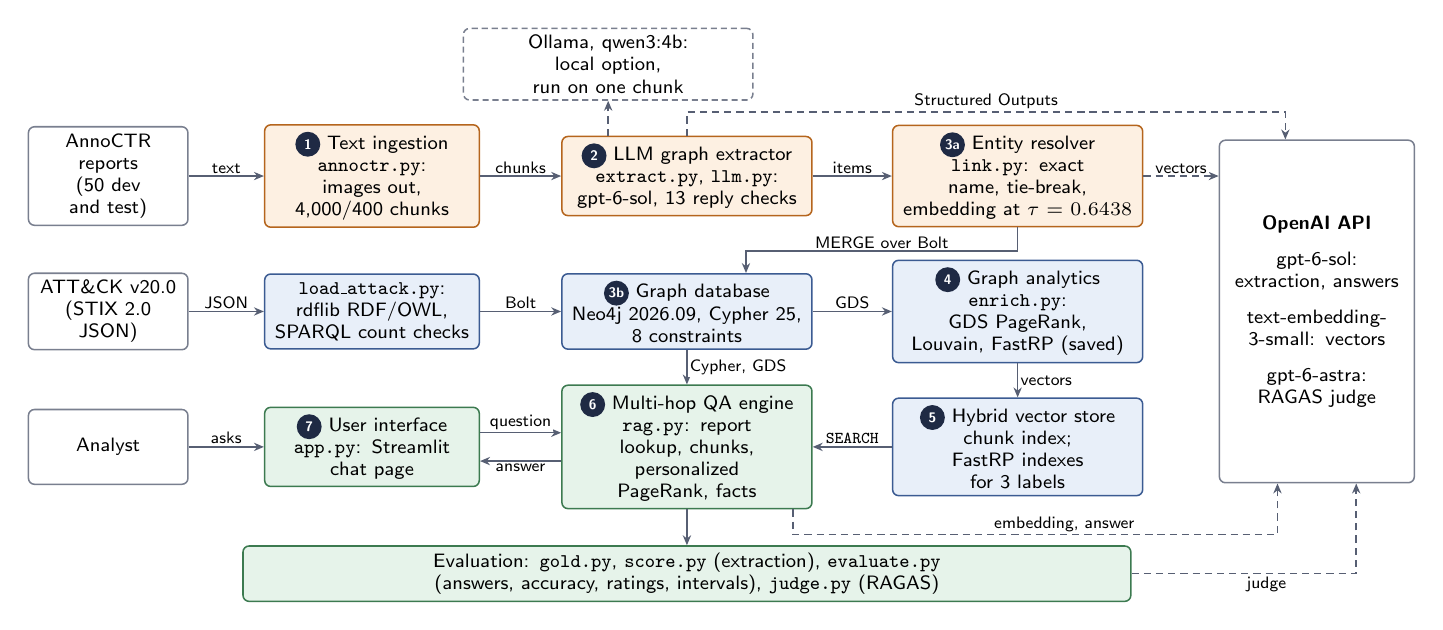
\begin{tikzpicture}[x=1cm, y=1cm]
\tikzset{c1/.style={text width=1.85cm, minimum height=0.95cm}, c2/.style={text width=2.55cm, minimum height=0.95cm},
  c3/.style={text width=3.0cm, minimum height=0.95cm}, call/.style={flow, dash pattern=on 2.6pt off 1.8pt}}
\node[plainbox, c1] (src) at (1.0,0) {AnnoCTR reports\\(50 dev and test)};
\node[txtbox, c2] (ing) at (4.35,0) {\badge{1} Text ingestion\\\code{annoctr.py}: images out,\\4,000/400 chunks};
\node[txtbox, c3] (ext) at (8.35,0) {\badge{2} LLM graph extractor\\\code{extract.py}, \code{llm.py}:\\gpt-6-sol, 13 reply checks};
\node[txtbox, c3] (ned) at (12.55,0) {\badge{3a} Entity resolver\\\code{link.py}: exact name, tie-break,\\embedding at $\tau = 0.6438$};
\node[plainbox, text width=2.3cm, minimum height=4.35cm] (oai) at (16.35,-1.72) {\textbf{OpenAI API}\\[5pt]gpt-6-sol:\\extraction, answers\\[5pt]text-embedding-\\3-small: vectors\\[5pt]gpt-6-astra:\\RAGAS judge};
\node[plainbox, dash pattern=on 2.2pt off 1.4pt, text width=3.5cm] (oll) at (7.35,1.42) {Ollama, qwen3:4b: local option,\\run on one chunk};
\node[plainbox, c1] (stix) at (1.0,-1.72) {ATT\&CK v20.0\\(STIX 2.0 JSON)};
\node[attbox, c2] (rdf) at (4.35,-1.72) {\code{load\_attack.py}:\\rdflib RDF/OWL,\\SPARQL count checks};
\node[attbox, c3] (neo) at (8.35,-1.72) {\badge{3b} Graph database\\Neo4j 2026.09, Cypher 25,\\8 constraints};
\node[attbox, c3] (emb) at (12.55,-1.72) {\badge{4} Graph analytics\\\code{enrich.py}: GDS PageRank,\\Louvain, FastRP (saved)};
\node[plainbox, c1] (an) at (1.0,-3.44) {Analyst};
\node[evalbox, c2] (ui) at (4.35,-3.44) {\badge{7} User interface\\\code{app.py}: Streamlit\\chat page};
\node[evalbox, c3] (qa) at (8.35,-3.44) {\badge{6} Multi-hop QA engine\\\code{rag.py}: report lookup, chunks,\\personalized PageRank, facts};
\node[attbox, c3] (vec) at (12.55,-3.44) {\badge{5} Hybrid vector store\\chunk index; FastRP indexes\\for 3 labels};
\node[evalbox, text width=11.1cm, minimum height=0.5cm] (ev) at (8.35,-5.05) {Evaluation: \code{gold.py}, \code{score.py} (extraction), \code{evaluate.py} (answers, accuracy, ratings, intervals), \code{judge.py} (RAGAS)};
\draw[flow] (src) -- node[elab, above]{text} (ing);
\draw[flow] (ing) -- node[elab, above]{chunks} (ext);
\draw[flow] (ext) -- node[elab, above]{items} (ned);
\draw[flow] (stix) -- node[elab, above]{JSON} (rdf);
\draw[flow] (rdf) -- node[elab, above]{Bolt} (neo);
\draw[flow] (neo) -- node[elab, above]{GDS} (emb);
\draw[flow] (ned.south) -- ++(0,-0.3) -| node[elab, pos=0.25, above]{MERGE over Bolt} ($(neo.north)+(0.75,0)$);
\draw[flow] (emb.south) -- node[elab, right]{vectors} (vec.north);
\draw[flow] (vec) -- node[elab, above]{\code{SEARCH}} (qa);
\draw[flow] (neo.south) -- node[elab, right]{Cypher, GDS} (qa.north);
\draw[flow] (an) -- node[elab, above]{asks} (ui);
\draw[flow] ($(ui.east)+(0,0.18)$) -- node[elab, above]{question} ($(qa.west)+(0,0.18)$);
\draw[flow] ($(qa.west)+(0,-0.18)$) -- node[elab, below]{answer} ($(ui.east)+(0,-0.18)$);
\draw[flow] (qa.south) -- (qa.south |- ev.north);
\draw[call] (ext.north) -- ++(0,0.3) -| node[elab, pos=0.25, above]{Structured Outputs} ($(oai.north)+(-0.4,0)$);
\draw[call] (ned) -- node[elab, above]{vectors} (ned -| oai.west);
\draw[call] ([xshift=-10mm]ext.north) -- ([xshift=-10mm]ext.north |- oll.south);
\draw[call] ($(qa.south east)+(-0.25,0)$) -- ++(0,-0.32) -| node[elab, pos=0.28, above]{embedding, answer} ($(oai.south)+(-0.5,0)$);
\draw[call] (ev.east) -| node[elab, pos=0.3, below]{judge} ($(oai.south)+(0.5,0)$);
\end{tikzpicture}
\caption{Architecture as built. Numbered boxes are the seven subsystems of the design: 1 text ingestion, 2 LLM graph extractor, 3a entity resolver, 3b graph database, 4 graph analytics, 5 hybrid vector store, 6 multi-hop question-answering (QA) engine, 7 user interface. Dashed arrows are calls to model services: the OpenAI application programming interface (API), reached over HTTPS (Hypertext Transfer Protocol Secure), whose replies are saved and reused, and Ollama, a local option for the extractor that was run on one chunk (Section~\ref{sec:llmext}). Bolt is Neo4j's network protocol.}\label{fig:arch}
\end{figure*}

Fig.~\ref{fig:arch} shows the pipeline. Report text and ATT\&CK enter on separate paths and meet in Neo4j through the entity resolver.

\subsection{Data and splits}
AnnoCTR (commit \code{d510b69}) splits its 120 reports into train (70), dev (16) and test (34). The gold standard, written by \code{gold.py} from the experts' links and mapped to ATT\&CK v20.0, holds 213 dev and 469 test (report, ATT\&CK entry) facts; the test facts are 327 techniques, 85 tactics, 13 groups and 44 software. Ten links to the revoked T1562 become T1685, and six links to ATT\&CK Mobile IDs are left out. The experts labeled parent techniques only: none of the 682 facts names a sub-technique. Train reports supply the prompt's two worked examples, dev reports set the linking threshold, and the test reports were extracted, linked and scored once. Linking cannot rely on names: only 288 of the 1,526 test mentions with an expert link have a text equal to an ATT\&CK name or alias, and 45.3\% describe a behavior without naming it.

\subsection{Text ingestion and normalization}
\code{annoctr.py} removes embedded base64 images (keeping their alt text) and cuts each report into 4,000-character chunks that overlap by 400 characters (dev 50, test 99 chunks), so any sentence of up to 400 characters that crosses a boundary is whole in one chunk. All text comparisons map typographic quotes and dashes to plain ones and collapse white space. On the ATT\&CK side, the loader drops revoked and deprecated objects (157 revoked-by mappings exist in v20.0), uses the version-20 names (the former Defense Evasion tactic is now Stealth and Defense Impairment), and checks the ATT\&CK file's \mbox{SHA-256} hash before reading it; the setup check compares all 124 data files with a committed list of hashes.

\subsection{LLM extraction: prompt, temperature and schema enforcement}\label{sec:llmext}
Each extraction request holds a system prompt, two worked examples (the openings of two train reports, with hand-written replies of 12 and 16 mentions) and the chunk. The prompt asks for one entry per place where the chunk names or describes a technique, tactic, group or software: the words copied exactly, the category, the ATT\&CK v20 name it denotes (a sub-technique as ``Parent: Sub-technique''), the whole evidence sentence and a confidence; then the ``uses'' relations between entries, referenced by local entry IDs (m1, m2, \ldots). Code builds every permanent identifier from the chunk's identifier and the model's local entry ID (Fig.~\ref{fig:example} cites \code{\ldots\#0/m18}). An excerpt of the prompt, with cuts marked [\ldots]:
\begin{lstlisting}
[...]
List one entry for each place where the chunk names or describes a concept:
[...]
- text: the words in the chunk that name or describe the concept, copied exactly
[...]
- attack_name: the concept's name in ATT&CK Enterprise version 20, spelled as ATT&CK spells it; for a sub-technique write "Parent technique: Sub-technique"; write "" when no ATT&CK entry fits
- evidence: the whole sentence of the chunk that contains the text, copied exactly
[...]
Copy text and evidence character for character from the chunk. Every entry must rest on the chunk's own words; use your knowledge of ATT&CK only to choose attack_name. [...]
\end{lstlisting}
The model is gpt-6-sol through OpenAI's Chat Completions application programming interface (API) with reasoning effort \emph{none}, temperature 0, seed 7 and at most 4,000 completion tokens; a reply cut off at that cap is requested once more with 8,000. Schema enforcement has two layers. Pydantic models compile to OpenAI Structured Outputs, a JSON schema the reply must follow; code then checks 13 drop reasons, each with its own counter: refusal, content filter, cut-off, invalid JSON, a repeated or empty entry, a text or evidence sentence not found in the chunk, a text not inside its evidence, a relation to a missing entry, a relation pointing the wrong way, categories that cannot use each other, and relation evidence not in the chunk. Separately, every reply is saved under the \mbox{SHA-256} hash of its request and replayed on reruns.

On the dev split all 50 replies were complete (980 mentions and 121 relations kept, \$1.13 at list price). On the test split 98 of 99 replies were complete; the one failure was a chunk holding a Markdown table of techniques, whose cells the model copied as evidence sentences until the reply hit both caps. The test run kept 1,818 mentions (962 technique, 138 tactic, 207 group, 511 software) and 178 relations, dropped 9 mentions (7 whose evidence sentence was not in the chunk) and 2 relations from complete replies, and used 389,031 input and 147,902 output tokens (\$2.25, 1,047\,s, 10.3\,s per reply on average). After the full runs, the same prompt ran once through Ollama with qwen3:4b on the project laptop's central processing unit (CPU; an Intel i7-1255U, with no usable graphics processing unit): the reply followed the schema but took 838.3\,s, about 100 times the 8.51\,s of gpt-6-sol on the same chunk, and only 1 of its 8 kept mentions named an ATT\&CK entry exactly. The local path works, but at that speed the 149 dev and test chunks would take about 35 hours on this laptop (estimated).

\subsection{Named entity disambiguation}\label{sec:ned}
\code{link.py} resolves each kept mention in four steps. (1) Normalize the names. (2) Look up the model's ATT\&CK name, then the mention text, among 2,927 keys (2,448 distinct ATT\&CK names and aliases plus 479 ``Parent: Sub-technique'' names) across all five ATT\&CK labels, never only the label the model guessed. (3) Settle a key shared by several entries (49 keys; ``Carbanak'' names a group and a piece of software) by the model's category and then by the named parent, never by an arbitrary pick. (4) Otherwise embed the model's name, the mention text and its evidence sentence with text-embedding-3-small and take the most similar ATT\&CK entry, compared as ``name: description''. A link is kept when it is exact or its cosine similarity reaches $\tau$, and the model's own confidence reaches $c$; any other mention becomes an Entity node. The pair $(\tau, c)$ was chosen on the dev reports from 4,554 candidates by the highest parent-level F1 (the harmonic mean of precision and recall against the gold facts, a sub-technique counting as its parent; Section~\ref{sec:eval}): $\tau = 0.6438$ and $c = 0.75$ raised dev F1 from 0.591 (at $\tau = 0.40$ with no cut-off) to 0.687, and both values were fixed before the test split was opened. On the test reports the linker made 1,169 exact links, 1 exact link with a tie broken by category and 43 embedding links, and left 605 mentions (33\%) as Entity nodes: 307 whose closest entry fell below $\tau$ and 298 whose model confidence fell below $c$, 250 of which had an exact-name match.

\subsection{Loading}
Writes use Cypher 25 \code{MERGE} in batches of 1,000, so a rerun changes nothing; reloading a report first removes its text-derived nodes and relationships, and every load is read back and counted (test: 34 of 34 reports, 99 chunks, 1,818 MENTIONS and 178 text USES edges).

% =====================================================================================================================
\section{Graph Data Science and Reasoning}\label{sec:gds}
\subsection{Projection and topology}
GDS 2026.09 runs on one undirected Cypher projection of the ATT\&CK part of the graph: the five ATT\&CK labels and the four relationship types as MITRE records them (\code{source = attack}), so that loading reports cannot change the results. GDS reports 1,785 nodes and 40,852 relationships (each of the 20,426 counted in both directions). Table~\ref{tab:topology} gives the topology, computed in Python from the same projection; its node and relationship counts and its Louvain modularity equal the GDS output. The graph is one connected component with a heavy-tailed degree distribution (Fig.~\ref{fig:degree}): the median entry has 12 relationships, while T1105 Ingress Tool Transfer has 504, of which 411 are USES from software and 90 USES from groups. No two entries are more than 6 hops apart, 88.1\% of ordered pairs are within 3 hops, and the 2-hop neighborhood of a single entry holds 623 entries on average (35\% of the graph), so retrieval ranks the neighborhood of a report's entities instead of taking it whole (Section~\ref{sec:retrieval}).

\begin{table}[t]\centering\footnotesize
\caption{Topology of the ATT\&CK projection (1,785 nodes)}\label{tab:topology}
\setlength{\tabcolsep}{3pt}
\begin{tabularx}{\linewidth}{@{}>{\raggedright\arraybackslash}X r@{}}
\toprule
Measure & Value\\
\midrule
Relationships (distinct node pairs; no parallels, no loops) & 20,426\\
Density (pairs / possible pairs) & 0.0128\\
Degree: mean; median; maximum (T1105) & 22.9; 12; 504\\
Mean degree: Technique; Tactic; Group; Software; Mitigation & 28.0; 58.7; 33.6; 15.2; 33.6\\
Connected components & 1\\
Average shortest path; diameter; radius (hops) & 2.76; 6; 4\\
Ordered node pairs within 3 hops & 88.1\%\\
Average local clustering coefficient & 0.100\\
Louvain: communities; modularity; levels & 6; 0.2953; 3\\
Spearman correlation of PageRank and degree & 0.983\\
\bottomrule
\end{tabularx}
\end{table}

\begin{figure}[t]\centering
\begin{tikzpicture}
\begin{axis}[width=\linewidth, height=4.1cm, xmode=log, ymode=log, xmin=1, xmax=600, ymin=0.0005, ymax=1.3,
  axis line style={draw=axisc, line width=0.5pt}, axis x line*=bottom, axis y line*=left,
  tick style={draw=axisc, line width=0.5pt}, grid=major, grid style={draw=gridc, line width=0.4pt},
  tick label style={font=\sffamily\scriptsize, text=ink2}, label style={font=\sffamily\scriptsize, text=ink2},
  xlabel={degree $k$ (relationships)}, ylabel={share with degree $\geq k$},
  ylabel style={yshift=-3pt}, xlabel style={yshift=2pt},
  legend style={font=\sffamily\tiny, draw=none, fill=none, at={(0.02,0.03)}, anchor=south west, row sep=-1.5pt},
  legend cell align=left, every axis plot/.append style={line width=0.85pt}]
\addplot[const plot, color=sysc] table[x=k, y=share] {data/degree_Technique.dat};
\addplot[const plot, color=basec, dashed] table[x=k, y=share] {data/degree_Software.dat};
\addplot[const plot, color=aquac, dash dot] table[x=k, y=share] {data/degree_Group.dat};
\addplot[const plot, color=yellowc, densely dotted] table[x=k, y=share] {data/degree_Mitigation.dat};
\addplot[const plot, color=magentac, dash pattern=on 3pt off 1pt on 1pt off 1pt on 1pt off 1pt] table[x=k, y=share] {data/degree_Tactic.dat};
\legend{Technique (706), Software (842), Group (178), Mitigation (44), Tactic (15)}
\end{axis}
\end{tikzpicture}
\caption{Share of each label's entries with at least $k$ relationships in the ATT\&CK projection (log scales). Techniques hold both the most low-degree entries (52.8\% have at most 10 relationships, against 42.5\% of software) and the hubs (38 have 100 or more, up to 504); software's tail is short (1.5\% have 50 or more; maximum 103).}\label{fig:degree}
\end{figure}

\subsection{Centrality}
Global PageRank (damping 0.85, one thread) ranks T1105 Ingress Tool Transfer (18.28), T1071.001 Web Protocols (14.98), T1082 System Information Discovery (14.83), T1059.003 Windows Command Shell (13.42) and T1083 File and Directory Discovery (13.18) highest. On this undirected graph PageRank follows degree closely (Spearman 0.983, with tied ranks averaged), so it measures how widely an entry is used more than any separate notion of authority (inference). The highest-ranked groups are Kimsuky, APT28 and APT29; software, Cobalt Strike, Empire and Mimikatz; mitigations, M1018 User Account Management, M1056 Pre-compromise and M1047 Audit. The scores, community numbers and FastRP vectors are saved to files and written to the ATT\&CK nodes on every machine; the chat page searches the FastRP vectors for similar entries, and retrieval uses the personalized variant of PageRank (Section~\ref{sec:retrieval}).

\subsection{Communities}
Louvain (GDS defaults, one thread; the result is saved to a file) found 6 communities with modularity 0.2953 in 3 levels. Table~\ref{tab:communities} lists their make-up. The communities follow kinds of entry and stages of an attack: malware with the techniques it implements; host techniques together with 36 of the 44 mitigations; hands-on intrusion groups with dual-use tools and lateral movement; command-and-control malware; pre-compromise reconnaissance and resource development; and impact. These readings are interpretations of the make-up, not measurements.

\begin{table}[t]\centering\footnotesize
\caption{Louvain communities (Te: techniques, Ta: tactics, G: groups, S: software, M: mitigations)}\label{tab:communities}
\setlength{\tabcolsep}{2.4pt}
\begin{tabularx}{\linewidth}{@{}r r >{\raggedright\arraybackslash}p{2.1cm} >{\raggedright\arraybackslash}X@{}}
\toprule
\# & Size & Te/Ta/G/S/M & Top tactics of its techniques; highest-PageRank technique, group, software\\
\midrule
1 & 560 & 76/0/42/442/0 & Stealth, Discovery; T1105, Gamaredon Group, InvisiMole\\
2 & 481 & 361/9/12/63/36 & Persistence, Stealth; T1036, APT29, Mini Shai-Hulud\\
3 & 228 & 66/2/73/85/2 & Discovery, Lateral Movement; T1059.001, APT41, Cobalt Strike\\
4 & 228 & 63/1/13/147/4 & Command and Control, Stealth; T1140, Lazarus Group, Emotet\\
5 & 156 & 100/2/37/16/1 & Resource Development, Reconnaissance; T1566.002, Kimsuky, PoisonIvy\\
6 & 132 & 40/1/1/89/1 & Impact, then Defense Impairment and Stealth (tied); T1112, Water Galura, DarkGate\\
\bottomrule
\end{tabularx}
\end{table}

\subsection{Graph embeddings}
FastRP \cite{chen2019} embeds each entry in 128 numbers from its 2- and 3-hop neighborhood (iteration weights 0, 1, 1; no self-influence; seed 42; one thread). Its random start depends on internal node identifiers, so the vectors are computed once and saved. The nearest group to G0129 Mustang Panda is G1014 LuminousMoth (Neo4j similarity 0.948, cosine 0.897), then LazyScripter (0.929) and Earth Lusca (0.928). The closeness comes from shared USES edges: 20 of LuminousMoth's 30 USES targets are also Mustang Panda's. ATT\&CK records a link between the two groups only in text (LuminousMoth's description reports that some researchers connect it with Mustang Panda, and Mustang Panda's aliases include LUMINOUS MOTH), not as an edge, so this is one example of the embedding placing related groups together, not a new finding.

\subsection{Path calculations and rule-based reasoning}\label{sec:rules}
\textbf{Multi-hop paths.} Each benchmark question (Section~\ref{sec:eval}) stores a Cypher query over its path pattern, run with the report's gold entries as parameters; all 24 return the reference answers in Neo4j. The query for the mitigation questions counts, for each mitigation, the report's techniques (\code{\$techniques}; for Q01, the 13 the experts labeled) that it addresses directly or through a sub-technique, and returns the mitigations with the highest count. Reformatted (the stored query starts with \code{CYPHER 25} and quotes every name in backticks):
\begin{lstlisting}
MATCH (m:Mitigation)-[:MITIGATES]->(:Technique)-[:SUBTECHNIQUE_OF*0..1]->(t:Technique)
WHERE t.attack_id IN $techniques
WITH m, collect(DISTINCT t.attack_id) AS addressed
WITH max(size(addressed)) AS most, collect({id: m.attack_id, addressed: addressed}) AS rows
UNWIND rows AS row WITH row, most WHERE size(row.addressed) = most
RETURN row.id AS answer, row.addressed AS support ORDER BY answer
\end{lstlisting}
\textbf{Hierarchy rule.} A relationship ATT\&CK records for a sub-technique also holds for its parent: $\mathit{USES}(x,s) \wedge \mathit{SUBTECHNIQUE\_OF}(s,t) \Rightarrow \mathit{USES}(x,t)$, and likewise for MITIGATES. The rule matters because 8,877 of ATT\&CK's 16,423 USES relationships to techniques point at sub-techniques, while the experts label parents only. Queries apply it with the variable-length step \code{-[:SUBTECHNIQUE\_OF*0..1]->}, and the scorer and the summary lines apply it at parent level. The rule writes no relationship, so every derived fact still cites a recorded edge. \textbf{Personalized PageRank} is the path computation made for each question (Section~\ref{sec:retrieval}).

% =====================================================================================================================
\section{LLM Integration and GraphRAG Performance}\label{sec:llm}
\subsection{Retrieval and prompt}\label{sec:retrieval}
\code{rag.py} answers a question in seven steps. (1) \emph{Report lookup}: a quoted span equal to a report's normalized title anchors that report; all 24 benchmark questions anchored exactly the reports they name. (2) \emph{Chunks}: the question's embedding selects up to 4 most similar chunks of the anchored reports by exact cosine (the chunk index serves questions that name no report). (3) \emph{Seeds}: every node the anchored reports mention. (4) \emph{Walk}: personalized PageRank \cite{haveliwala2002} on an undirected projection of the whole graph (2,258 nodes; USES from ATT\&CK and from text, SUBTECHNIQUE\_OF, PART\_OF\_TACTIC, MITIGATES), damping 0.85, at most 40 iterations, one thread, with the seeds as source nodes; the 200 best nodes are kept. HippoRAG \cite{gutierrez2024} uses a similar walk for multi-hop retrieval. (5) \emph{Summary lines}: report lines list each anchored report's entries by kind; then Cypher counts, for every ATT\&CK entry one relationship from those entries and each relationship type, how many of the entries it links to by ATT\&CK relationships (a sub-technique link counting for its parent), with one edge ID per counted entry, so the model reads counts instead of computing them. At most 40 node lines are kept, taken in turn from MITIGATES, USES and PART\_OF\_TACTIC, highest count first; PageRank only breaks ties, so a line may describe a node outside the 200 kept (200 of the 960 node lines for the 24 questions did). (6) \emph{Facts}: up to 40 mention facts and 60 relationship facts among the kept nodes, seed to seed first, then one and two steps out, taken in turn from each type. (7) \emph{Answer}: gpt-6-sol (reasoning effort \emph{none}, temperature 0, seed 7, at most 1,500 tokens) with the system prompt below and a user message holding the question, the chunks and, for GraphRAG only, the facts. Code parses every \code{[chunk:\ldots]} and \code{[edge:\ldots]} citation and flags any identifier that was not in the context (a citation-ID validity check: it shows that the cited item was supplied, not that it supports the claim). The text-only baseline runs steps 1, 2 and 7 with the same chunks, so the two systems differ only in the graph context.
\begin{lstlisting}
You answer questions about cyber threat reports. Use only the context given after the question: report chunks, and knowledge-graph facts when there are any. After every statement, cite in square brackets the IDs of the chunks or facts that support it, exactly as they appear in the context, for example [chunk:report_2020-01-01_example#0] or [edge:attack:MITIGATES:M1040:T1055]. Do not use knowledge from outside the context. If the context does not answer the question, say what is missing.
\end{lstlisting}

\subsection{An answer and its provenance}
Fig.~\ref{fig:example} shows question Q10 answered by both systems, with each GraphRAG citation resolved to its record. The baseline's chunks name APT-C-36 and njRAT but hold no ATT\&CK relationship, so the baseline declines. GraphRAG answers from the ATT\&CK edge \code{USES(G0099, S0385)} and the two mention edges that tie the report to the group and to njRAT. LimeRAT, which the report also names, has no ATT\&CK entry; its mention became an Entity node (\emph{unlinked}, best embedding match below $\tau$), and the answer notes that the supplied ATT\&CK relationship covers njRAT only. On the chat page (Fig.~\ref{fig:arch}, box~7), each answer appears beside the baseline's with its citation check and the context the model saw, and GraphRAG's cited relationships and chunks are drawn as a graph, read from Neo4j by their edge IDs; the session's earlier questions and answers stay on the page.

\begin{figure}[t]\centering
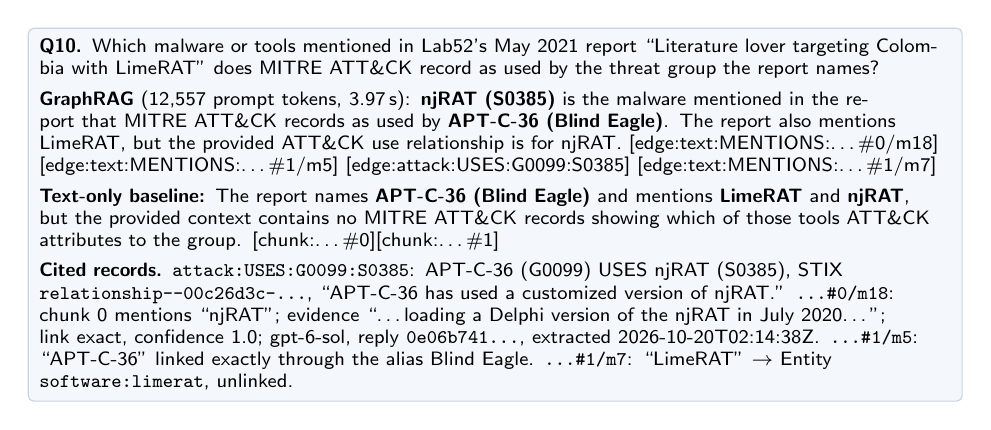
\begin{tikzpicture}
\node[draw=rulec, fill=shade, rounded corners=2pt, text width=0.955\linewidth, inner sep=4pt, align=left, font=\sffamily\scriptsize] {%
\textbf{Q10.} Which malware or tools mentioned in Lab52's May 2021 report ``Literature lover targeting Colombia with LimeRAT'' does MITRE ATT\&CK record as used by the threat group the report names?\\[3pt]
\textbf{GraphRAG} (12,557 prompt tokens, 3.97\,s): \textbf{njRAT (S0385)} is the malware mentioned in the report that MITRE ATT\&CK records as used by \textbf{APT-C-36 (Blind Eagle)}. The report also mentions LimeRAT, but the provided ATT\&CK use relationship is for njRAT. [edge:text:MENTIONS:\ldots\#0/m18] [edge:text:MENTIONS:\ldots\#1/m5] [edge:attack:USES:G0099:S0385] [edge:text:MENTIONS:\ldots\#1/m7]\\[3pt]
\textbf{Text-only baseline:} The report names \textbf{APT-C-36 (Blind Eagle)} and mentions \textbf{LimeRAT} and \textbf{njRAT}, but the provided context contains no MITRE ATT\&CK records showing which of those tools ATT\&CK attributes to the group. [chunk:\ldots\#0][chunk:\ldots\#1]\\[3pt]
\textbf{Cited records.} \code{attack:USES:G0099:S0385}: APT-C-36 (G0099) USES njRAT (S0385), STIX \code{relationship-{}-00c26d3c-\ldots}, ``APT-C-36 has used a customized version of njRAT.''\enspace
\code{\ldots\#0/m18}: chunk 0 mentions ``njRAT''; evidence ``\ldots loading a Delphi version of the njRAT in July 2020\ldots''; link exact, confidence 1.0; gpt-6-sol, reply \code{0e06b741\ldots}, extracted 2026-10-20T02:14:38Z.\enspace
\code{\ldots\#1/m5}: ``APT-C-36'' linked exactly through the alias Blind Eagle.\enspace
\code{\ldots\#1/m7}: ``LimeRAT'' $\rightarrow$ Entity \code{software:limerat}, unlinked.};
\end{tikzpicture}
\caption{Question Q10: both answers (verbatim, with their Markdown bold shown as bold and the report identifier shortened to \ldots) and the records behind GraphRAG's four citations, as stored on the edges (the ATT\&CK description as cleaned for the model).}\label{fig:example}
\end{figure}

\subsection{Effect of the graph context}
The assignment asks how graph context improves factual accuracy, reduces hallucination and provides provenance; over the 24 benchmark questions (details in Section~\ref{sec:eval}), the measurements answer each in turn. \emph{Factual accuracy}: the mean F1 of the ATT\&CK IDs an answer names against the reference rises from 0.125 to 0.492 (+0.367, 95\% interval [0.208, 0.530]), recall from 0.129 to 0.571, and blind-rated Completeness from 1.38 to 3.50 of 5; blind-rated Factuality, however, falls from 4.63 to 3.17, because GraphRAG states items, some of them wrong, where the baseline mostly states that it cannot answer. \emph{Hallucination}, measured as answer statements the RAGAS judge found unsupported by the answer's own context, is rare in both systems (3 of 167 statements against 2 of 121; difference +0.001 [$-0.030$, 0.032]), so the graph does not measurably reduce it. \emph{Provenance}: GraphRAG made 229 citations (222 counting each ID once per answer), every answer cited at least one item, and every cited identifier was in the context; each resolves to an edge or chunk as in Fig.~\ref{fig:example}. Split at sentence-final punctuation, 58 of the 68 sentences in GraphRAG's answers carry their own citation, and 7 of the other 10 introduce a list whose items are cited. The graph context thus changes what the model can say more than how carefully it says it (inference). The price is a larger context (median 13,553 against 2,642 prompt tokens), a mean of \$0.0304 against \$0.0069 per question at list price, and a median of 4.10\,s against 2.19\,s end to end.

% =====================================================================================================================
\section{Evaluation and Discussion}\label{sec:eval}
\subsection{Benchmark and protocol}
\textbf{Questions.} \code{eval\_queries.json} holds 24 multi-hop questions in 10 patterns about 20 test reports (Table~\ref{tab:patterns}), each naming its report by title. Answers (1 to 6 items) were computed in Python from the gold facts and ATT\&CK v20.0, never from the system's graph; each was recomputed by its Cypher query in Neo4j, all 24 were recomputed by an independent reimplementation, and three were compared item by item with attack.mitre.org. Each question also stores a reference answer in words.

\begin{table}[t]\centering\footnotesize
\caption{Benchmark question patterns (24 questions, 20 test reports; 10 patterns in 8 rows, as two rows each join two related patterns)}\label{tab:patterns}
\setlength{\tabcolsep}{3pt}
\begin{tabularx}{\linewidth}{@{}>{\raggedright\arraybackslash}p{2.75cm} r >{\raggedright\arraybackslash}X@{}}
\toprule
Pattern & $n$ & Path (Report $\rightarrow$ \ldots)\\
\midrule
Top mitigations & 5 & MENTIONS Technique, hierarchy, $\leftarrow$MITIGATES Mitigation, counted\\
Tactics & 4 & MENTIONS Technique $\rightarrow$PART\_OF\_TACTIC Tactic\\
Group's software (incl.\ inverse) & 3 & MENTIONS Group $\rightarrow$USES Software $\leftarrow$MENTIONS Report\\
Group's / software's techniques & 5 & MENTIONS Group or Software $\rightarrow$USES Technique, hierarchy, $\leftarrow$MENTIONS Report\\
Group using most techniques & 1 & as above, counted per group\\
Techniques a software lacks & 1 & MENTIONS Technique with no USES path from the software\\
Shared techniques & 3 & Report A $\rightarrow$MENTIONS Technique $\leftarrow$MENTIONS Report B\\
Groups using every technique & 2 & MENTIONS Technique, hierarchy, $\leftarrow$USES Group, for all\\
\bottomrule
\end{tabularx}
\end{table}

\textbf{Measures.} \emph{Extraction and linking}: precision, recall and F1 $= 2TP/(2TP+FP+FN)$, with $TP$, $FP$ and $FN$ the true positives, false positives and false negatives, of (report, ATT\&CK ID) facts against the gold, pooled over the 34 test reports, at sub-technique level and at parent level (a sub-technique counts as its parent, as the experts label parents), beside an exact-name baseline that links every ATT\&CK name or alias of a technique, sub-technique, tactic, group or software entry (2,407 names) found in a report as a whole word, ignoring case. \emph{Answer-ID accuracy}: per question, the precision, recall and F1 of the IDs of the asked kind that the answer names outside its citations, averaged over the questions. \emph{Blind human ratings}: one rater, the team's only member, who built the system, scored all 48 answers from 1 to 5 for Factuality, Completeness (the share of reference items given) and Coherence against the reference answer and anchored descriptions of each score; each question's two answers appeared as A and B in an order drawn with a fixed seed, with citations replaced by neutral numbers and the cited texts listed in one format for both systems. \emph{RAGAS} 0.4.3 \cite{es2024}: Faithfulness, AnswerRelevancy and ContextRecall, judged by gpt-6-astra at reasoning effort \emph{low} (288 judge calls, \$14.17 at list price). \emph{Hallucination rate}: the share of answer statements the faithfulness verdicts mark unsupported, pooled over statements. \emph{Operations}: seconds per stage, tokens and cost per question. \emph{Intervals}: 95\% percentile bootstrap \cite{efron1993}, 10,000 resamples with a fixed seed, resampling the 24 questions for answer measures (both systems on the same draws) and the 34 test reports for extraction.

\subsection{Extraction and linking}
\begin{figure}[t]\centering
\begin{tikzpicture}
\begin{axis}[dotchart, width=0.9\linewidth, height=3.6cm, xmin=0, xmax=1, ymin=-0.55, ymax=3.55, xtick={0,0.2,...,1},
  ytick={0,1,2,3}, yticklabels={{F1, sub-technique},{F1, parent},{Recall, parent},{Precision, parent}},
  xticklabel style={/pgf/number format/fixed}, title={Extraction and linking, 34 test reports (95\% intervals)},
  legend style={at={(0.42,-0.24)}, anchor=north, legend columns=2, draw=none, font=\sffamily\scriptsize,
  /tikz/every even column/.append style={column sep=8pt}}]
\addplot+[sysmark] table[x=a, y expr=\thisrow{y}+0.15, x error minus=am, x error plus=ap] {data/extraction.dat};
\addplot+[basemark] table[x=b, y expr=\thisrow{y}-0.15, x error minus=bm, x error plus=bp] {data/extraction.dat};
\legend{LLM extraction and linking, exact-name baseline}
\end{axis}
\end{tikzpicture}
\caption{Entity extraction and linking against the experts' 469 test facts.}\label{fig:extraction}
\end{figure}

At parent level the system reaches precision 0.756, recall 0.667 and F1 0.709 [0.661, 0.752], against 0.403, 0.488 and 0.442 [0.342, 0.528] for exact-name matching, a difference of +0.267 [0.172, 0.363] (Fig.~\ref{fig:extraction}). Most of the baseline's false links come from ATT\&CK names that are everyday words: 300 of its 339 false facts come only from one-word names, and 143 only from ``at'', ``malware'', ``server'', ``software'' and ``credentials'', which link wrongly in 28, 27, 15, 14 and 13 reports. By kind, the system scores F1 0.894 on software, 0.813 on groups, 0.662 on tactics and 0.687 on techniques (baseline: 0.476, 0.647, 0.545 and 0.398); tactics and techniques score lowest, plausibly because many of their mentions are implicit (inference). At sub-technique level F1 is 0.542, since every sub-technique link counts against parent-only gold. In the report with the one cut-off chunk, 24 of the 48 gold facts are labeled only inside that chunk; over all reports, 21 of the 156 parent-level misses are labeled only inside chunks that yielded no mentions. For context only: the AnnoCTR paper's best document-level F1 when its systems choose the sentences themselves is 56.6 for techniques (a fine-tuned sentence classifier selects the sentences that describe a technique, then a generative linker links them) and 47.7 for tactics (the linker run on every sentence with a negative class), and 65.7 and 84.2 when the sentences the experts annotated are given \cite[Table~9]{lange2024}. The settings differ (fine-tuned linkers against a prompted LLM; their technique and tactic scores against our parent-level facts), so the numbers do not rank the systems.

\subsection{Answers}
\begin{figure*}[t]\centering
\begin{tikzpicture}
\begin{axis}[dotchart, name=human, width=0.40\textwidth, height=4.0cm, xmin=1, xmax=5, ymin=-0.55, ymax=2.55,
  xtick={1,2,3,4,5}, ytick={0,1,2}, yticklabels={Coherence,Completeness,Factuality},
  title={(a) Blind human ratings, 1 to 5}]
\addplot+[sysmark] table[x=a, y expr=\thisrow{y}+0.22, x error minus=am, x error plus=ap] {data/human.dat};
\addplot+[basemark] table[x=b, y expr=\thisrow{y}-0.22, x error minus=bm, x error plus=bp] {data/human.dat};
\end{axis}
\begin{axis}[dotchart, name=auto, at={($(human.south east)+(3.7cm,0)$)}, anchor=south west, width=0.45\textwidth,
  height=4.0cm, xmin=0, xmax=1, ymin=-0.55, ymax=5.55, xtick={0,0.2,...,1}, xticklabel style={/pgf/number format/fixed},
  ytick={0,1,2,3,4,5},
  yticklabels={Hallucination rate,{RAGAS context recall},{RAGAS answer relevancy},{RAGAS faithfulness},{Answer-ID recall},{Answer-ID F1}},
  title={(b) Automatic measures, 0 to 1}]
\addplot+[sysmark] table[x=a, y expr=\thisrow{y}+0.22, x error minus=am, x error plus=ap] {data/automatic.dat};
\addplot+[basemark] table[x=b, y expr=\thisrow{y}-0.22, x error minus=bm, x error plus=bp] {data/automatic.dat};
\end{axis}
\node[anchor=north, font=\sffamily\scriptsize, inner sep=0pt] at ($(human.south west)!0.5!(auto.south east)+(0,-0.55cm)$) {%
  \tikz[baseline=-0.6ex]{\draw[sysc, line width=0.9pt] (0,0) -- (0.5,0); \fill[sysc] (0.25,0) circle (1.7pt);}~GraphRAG\qquad
  \tikz[baseline=-0.6ex]{\draw[basec, line width=0.9pt] (0,0) -- (0.5,0); \draw[basec, line width=0.9pt, fill=white] (0.25,0) circle (1.7pt);}~text-only baseline};
\end{tikzpicture}
\caption{Answer quality on the 24 benchmark questions: means with 95\% bootstrap intervals.}\label{fig:answers}
\end{figure*}

\begin{table}[t]\centering\footnotesize
\caption{Answer results: means over the 24 questions, except as noted for precision and the hallucination rate; difference GraphRAG $-$ baseline with 95\% interval}\label{tab:answers}
\setlength{\tabcolsep}{2.5pt}
\begin{tabularx}{\linewidth}{@{}>{\raggedright\arraybackslash}X r r r@{}}
\toprule
Measure & GraphRAG & Baseline & Difference\\
\midrule
Answer-ID F1 & 0.492 & 0.125 & +0.367 [0.208, 0.530]\\
Answer-ID recall & 0.571 & 0.129 & +0.442 [0.271, 0.617]\\
Answer-ID precision$^{a}$ & 0.563 & 0.781 & --\\
Factuality (1--5) & 3.17 & 4.63 & $-$1.46 [$-$2.08, $-$0.79]\\
Completeness (1--5) & 3.50 & 1.38 & +2.13 [1.50, 2.75]\\
Coherence (1--5) & 4.88 & 5.00 & $-$0.13 [$-$0.33, 0.00]\\
Sum of the three (3--15) & 11.54 & 11.00 & +0.54 [$-$0.38, 1.46]\\
RAGAS faithfulness & 0.976 & 0.987 & $-$0.011 [$-$0.045, 0.021]\\
RAGAS answer relevancy & 0.737 & 0.169 & +0.568 [0.442, 0.685]\\
RAGAS context recall & 0.367 & 0.051 & +0.316 [0.210, 0.428]\\
Hallucination rate$^{b}$ & 0.018 & 0.017 & +0.001 [$-$0.030, 0.032]\\
\bottomrule
\multicolumn{4}{@{}p{\linewidth}@{}}{\scriptsize $^{a}$Over the answers naming an ID of the asked kind: 21 GraphRAG, 4 baseline. $^{b}$Unsupported statements, pooled: 3 of 167 and 2 of 121. Per question, GraphRAG wins, ties and loses 2/4/18 on Factuality, 18/6/0 on Completeness, 0/22/2 on Coherence and 13/1/10 on the sum.}\\
\end{tabularx}
\end{table}

Table~\ref{tab:answers} and Fig.~\ref{fig:answers} give the results. Every measure of how much of the question an answer covers favors GraphRAG with an interval that excludes zero: answer-ID F1 and recall, Completeness, answer relevancy and context recall. Factuality favors the baseline, also with an interval that excludes zero. Faithfulness, the hallucination rate and Coherence do not separate the systems, and neither does the sum of the three human criteria (+0.54 [$-$0.38, 1.46]). The baseline's high Factuality comes from declining: it declined in 21 of its 24 answers, all but the three shared-technique questions, which the report texts can answer and which give most of its non-zero accuracy. All 21 were rated Completeness 1 and 19 of them Factuality 5, since a true statement that the context lacks the information is factual; RAGAS gave 19 of the 21 an answer relevancy of 0, the score for a noncommittal answer (Q11 and Q12, which name the report's groups and software before declining, scored 0.78 and 0.66).

\textbf{Operations.} The answer call dominates the time (median 3.33\,s for GraphRAG); report lookup, chunk search, seeds, personalized PageRank (median 0.18\,s) and the fact queries take a median of 0.77\,s together, under a second for 20 of the 24 questions and at most 4.86\,s (Q01, whose chunk stage took 3.14\,s; Table~\ref{tab:ops}). Both systems meet the design target of a median under 10\,s. All OpenAI use for the project cost about \$18.60 at list price: \$3.43 for extraction (including an early trial), about \$0.08 for development questions, \$0.90 for the 48 benchmark answers and \$14.17 for the RAGAS judge.

\begin{table}[t]\centering\footnotesize
\caption{Operations per question: median (maximum), except cost, a mean (total), and citations, a total over the 24 answers}\label{tab:ops}
\setlength{\tabcolsep}{3pt}
\begin{tabularx}{\linewidth}{@{}>{\raggedright\arraybackslash}X r r@{}}
\toprule
 & GraphRAG & Baseline\\
\midrule
Lookup, chunks, seeds (s) & 0.01, 0.25, 0.02 & 0.01, 0.02, --\\
Personalized PageRank; facts (s) & 0.18; 0.26 & --\\
Answer call (s) & 3.33 (6.70) & 2.16 (3.35)\\
End to end (s) & 4.10 (8.15) & 2.19 (3.38)\\
Prompt tokens & 13,553 (22,595) & 2,642 (4,744)\\
Cost at list price: mean (total, 24) & \$0.0304 (\$0.73) & \$0.0069 (\$0.17)\\
Citations, all in context (each ID once per answer) & 229 (222) & 66 (46)\\
\bottomrule
\end{tabularx}
\end{table}

\subsection{Error analysis}
\textbf{GraphRAG's answers follow its graph.} In the five mitigation questions, every GraphRAG answer named the mitigations with the highest count in its own summary lines. Where the graph's counts put the reference on top (Q03, Q04, Q05, and M1040 in Q02), the answer contained it. In Q01 the system linked 14 parent techniques against the experts' 13, sharing 9: it added T1105, T1204, T1543, T1547 and T1555 and missed T1001, T1114, T1189 and T1606. The added techniques lift M1018 and M1026 to 6, above the reference M1047 at 5, and the answer named M1018 and M1026. Three answers (Q02, Q04, Q05) also named mitigations below the top count, which costs precision. Some added links may be correct links the experts did not make: the gold holds one annotator's labels, and when the AnnoCTR authors had a second professional label techniques, the two sets agreed with an average F1 of 54\%, a figure they say is not a proper agreement study and likely underestimates agreement \cite{lange2024}.

\textbf{Faithful but wrong.} GraphRAG's statements are supported by its context (faithfulness 0.976) while its Factuality is lower, so its wrong items most likely come from the context itself, that is, from the graph the extraction built (parent-level precision 0.756), whose links the summary lines count (inference). Q01 is the example: the judge found every statement supported (faithfulness 1.00) while the reference answer is M1047.

\textbf{Measure artifacts.} The answer-ID measure credits listing: the baseline's Q14 answer says it cannot determine the techniques the group uses, then lists eight techniques from the report, three of them reference items, and earns recall 0.75, while the rater scored it Completeness 1. RAGAS's verdict step judges each statement without the question: GraphRAG's Q15 statement that its facts ``support Cobalt Group (G0080) as an answer to the question'' was marked unsupported for that reason alone.

\subsection{Limitations}
(1) One rater, who built the system, gives no agreement statistic, and the kind of evidence an answer cites can hint at its system. (2) 24 questions over 20 reports give wide intervals, and the patterns are unevenly represented. (3) The judge (gpt-6-astra) and the answering model (gpt-6-sol) both come from OpenAI's GPT-6 family (GPT: Generative Pre-trained Transformer), and judge models can favor text like their own \cite{zheng2023,panickssery2024,wataoka2024}; both systems share them, which protects the comparison more than the absolute scores. (4) The gold holds one annotator's labels, so a correct link outside it counts as an error (in one dev report, the name APT27 links to G0027, whose ATT\&CK aliases include it, while the expert did not link it to ATT\&CK). (5) The ``uses'' relations extracted from text are loaded but not scored, because no expert labels exist for them. (6) The caps of 40 summary lines and 60 relationship facts can drop a needed line. (7) Repeatability rests on the saved replies; a new request at temperature 0 with a fixed seed is not guaranteed to return the same reply. (8) The local-model path was shown on one chunk only. (9) The citation check shows that cited identifiers were supplied, not that they support the statement, and 10 of GraphRAG's 68 answer sentences carry no citation of their own.

\subsection{Future work}
Extraction and linking quality is the lever the error analysis points to (interpretation). A fine-tuned sentence classifier that selects the sentences describing a technique before linking, the step behind AnnoCTR's best technique score without given sentences \cite{lange2024}, could raise recall on implicit mentions, and table-aware chunking could recover the cut-off table chunk. Answers could commit to the Cypher-computed top count instead of restating counts in prose, which could remove the extra mitigations seen in Q02, Q04 and Q05. A larger benchmark with several raters would narrow the intervals, and expert labels for ``uses'' relations would let the extracted relations be scored.

% =====================================================================================================================
\section{Conclusion}
Joining threat reports to ATT\&CK in one knowledge graph lets a language model answer multi-hop CTI questions that a text-only pipeline declines, with citations that trace its statements to report sentences and ATT\&CK relationships through edge identifiers. The measured gains are in coverage: answer-ID F1 0.492 against 0.125 and Completeness 3.50 against 1.38. The measured cost is lower rated Factuality (3.17 against 4.63) than a baseline that mostly abstains, and the error analysis indicates that the answers follow the graph's extraction and linking (parent-level F1 0.709), mistakes included (inference). Faithfulness to the context is high (0.98 and 0.99) and unsupported statements are rare (under 2\%) in both systems, with no measurable difference.

\IEEEtriggeratref{12}
\begin{thebibliography}{99}
\footnotesize
\bibitem{lange2024} L.~Lange, M.~M\"uller, G.~Haratinezhad Torbati, D.~Milchevski, P.~Grau, S.~Pujari, and A.~Friedrich, ``AnnoCTR: A dataset for detecting and linking entities, tactics, and techniques in cyber threat reports,'' in \emph{Proc. LREC-COLING 2024}, Torino, Italy, 2024, pp.~1147--1160.
\bibitem{strom2020} B.~Strom, A.~Applebaum, D.~Miller, K.~Nickels, A.~Pennington, and C.~Thomas, ``MITRE ATT\&CK: Design and philosophy,'' The MITRE Corporation, Tech. Rep., Mar. 2020.
\bibitem{lewis2020} P.~Lewis \emph{et al.}, ``Retrieval-augmented generation for knowledge-intensive NLP tasks,'' in \emph{Advances in Neural Information Processing Systems 33}, 2020, pp.~9459--9474.
\bibitem{edge2024} D.~Edge \emph{et al.}, ``From local to global: A graph RAG approach to query-focused summarization,'' arXiv:2404.16130, 2024.
\bibitem{gutierrez2024} B.~Jim\'enez Guti\'errez, Y.~Shu, Y.~Gu, M.~Yasunaga, and Y.~Su, ``HippoRAG: Neurobiologically inspired long-term memory for large language models,'' in \emph{Advances in Neural Information Processing Systems 37}, 2024.
\bibitem{peng2024} B.~Peng \emph{et al.}, ``Graph retrieval-augmented generation: A survey,'' arXiv:2408.08921, 2024.
\bibitem{haveliwala2002} T.~H. Haveliwala, ``Topic-sensitive PageRank,'' in \emph{Proc. 11th Int. World Wide Web Conf. (WWW)}, Honolulu, HI, USA, 2002.
\bibitem{brin1998} S.~Brin and L.~Page, ``The anatomy of a large-scale hypertextual web search engine,'' \emph{Computer Networks}, vol.~30, pp.~107--117, 1998.
\bibitem{blondel2008} V.~D. Blondel, J.-L. Guillaume, R.~Lambiotte, and E.~Lefebvre, ``Fast unfolding of communities in large networks,'' \emph{J. Stat. Mech.}, vol.~2008, P10008, 2008.
\bibitem{chen2019} H.~Chen, S.~F. Sultan, Y.~Tian, M.~Chen, and S.~Skiena, ``Fast and accurate network embeddings via very sparse random projection,'' in \emph{Proc. 28th ACM CIKM}, 2019.
\bibitem{es2024} S.~Es, J.~James, L.~Espinosa Anke, and S.~Schockaert, ``RAGAs: Automated evaluation of retrieval augmented generation,'' in \emph{Proc. EACL 2024: System Demonstrations}, 2024, pp.~150--158.
\bibitem{efron1993} B.~Efron and R.~J. Tibshirani, \emph{An Introduction to the Bootstrap}. New York, NY, USA: Chapman \& Hall, 1993.
\bibitem{rdf11} R.~Cyganiak, D.~Wood, and M.~Lanthaler, Eds., ``RDF 1.1 concepts and abstract syntax,'' W3C Recommendation, Feb. 2014.
\bibitem{owl2} W3C OWL Working Group, ``OWL 2 Web Ontology Language document overview (second edition),'' W3C Recommendation, Dec. 2012.
\bibitem{malkov2020} Y.~A. Malkov and D.~A. Yashunin, ``Efficient and robust approximate nearest neighbor search using hierarchical navigable small world graphs,'' \emph{IEEE Trans. Pattern Anal. Mach. Intell.}, vol.~42, no.~4, pp.~824--836, 2020.
\bibitem{zheng2023} L.~Zheng \emph{et al.}, ``Judging LLM-as-a-judge with MT-Bench and Chatbot Arena,'' in \emph{Advances in Neural Information Processing Systems 36, Datasets and Benchmarks Track}, 2023.
\bibitem{panickssery2024} A.~Panickssery, S.~R. Bowman, and S.~Feng, ``LLM evaluators recognize and favor their own generations,'' in \emph{Advances in Neural Information Processing Systems 37}, 2024.
\bibitem{wataoka2024} K.~Wataoka, T.~Takahashi, and R.~Ri, ``Self-preference bias in LLM-as-a-judge,'' arXiv:2410.21819, 2024.
\end{thebibliography}

\end{document}
